\section{Materials and Methods}

\subsection{Participants}
A total of 23 right-handed subjects took part in the experiment (9 females, 14 males, $24 \pm 4.6$ years old). All subjects are non-smokers and without respiration problems. According to their self-reports, none had a history of injury in the olfactory bulb or incapability of smelling. Subjects were informed about the experimental protocol and the purpose of the study. During the experiment, subjects were seated in a comfortable chair with recording devices. None of the participants in experiment were wearing perfumed products on the day of experiment. A payback of 50CHF was offered to each subject after the experiment. 

\subsection{Experimental Setup}
An EGI's Geodesic EEG system (GES) 300 was used to record, amplify and digitalize the EEG signals. EEG signals were recorded from a 256-channel EEG Net Amps 300 cap with sampling frequency of 250Hz.  
\subsection{Experimental Protocol}
10 different odours were provided for the experiment, including rose water, lavender oil, jasmine oil, chocolate powder, mint oil, valerian pills, garlic powder, star anise, rotten cooked cauliflower and baby shampoo. The odorants were placed inside covered bottles so as to avoid effects of their visual characteristics.  

Subjects were asked to close their eyes and breath normally while the experimenter was moving bottles with different odorants towards them to smell. Subjects were not informed of the name of the odour during experiment. The experiment consisted of four runs. During each run, after a "smell" command, the experimenter was randomly coosing a bottle with an odor to place it under the subject's nose (1-2 cm under both nostrils) and keep it there for about 10 seconds, constituting a single trial. This process was repeated 15 times with the same odour resulting in 15 single trials. This repetition was carefully in done to ensure that sufficient number of single trials will be created for further data analysis. The time between two single trials of the same odour was set to 10 seconds in order to avoid adaptation and subject's fatigue. After one run was performed, the subjects were given two minutes break in order to forget the odour (to avoid masking effect) and in order for the odour to be evacuated. During this break, the subjects were asked to rate the odour in terms of pleasantness, in a scale from 0 to 10, ranging from extremely unpleasant to extremely pleasant for pleasantness. After this break another odour was randomly selected and the same procedure was repeated until all 10 odours were presented.    

\subsection{Pre-processing of EEG Signals}
After the pre-cleaning and synchronisation of recorded EEG signals by GES-300 system, a total of 12 seconds EEG segment is kept for each trial. It contains 6 seconds of baseline (resting state) and 6 seconds of active (odour perception). Signals from 40 electrodes which are placed on face muscles and around eyes are rejected in order to reduce muscle and eye movement artifacts. Signals from the remaining 216 electrodes are kept for further analysis. 

A bandpass filter (4th order butterworth) is applied for the EEG signals with pass-band 0-50Hz. Small laplacian filter is applied for each electrode in order to reduce volume conduction effects~\cite{wolters2007volume}. Eye-movement artifacts are rejected manually by using Independent Component Analysis (funcitons are provided by EEGLAB\copyright~ toolbox~\cite{luck2014introduction}). 

\subsection{Construction of Brain Networks}
Brain connectivity refers to a patter of anatomical links ("anatomical connectivity") or of statistical dependencies (functional connectivity) between neural assemblies. The connectivity pattern is formed by structural links such as synapses or represented by statistical or calsal relationships measured as cross-correlation, coherence or information flow~\cite{sporns2007brain}. Brain connectivity is a crucial concept to elucidate how neural networks process information. In this paper, we focus on the study of functional connectivity and utilise this kind of connectivity to interpret how brain functions during the perception of pleasant and unpleasant odours. 

A neurophysiological concept of functional connectivity is introduced by A.A Fingelkurts~\cite{fingelkurts2005functional}, which uses the notion of neural assemblies, as well as local and remote level of descriptions. According to Fingelkurts' concept, functional connectivity is described as the mechanism for the coordination of activity between different neural assemblies in order to achieve a complex cognitive task or perceptual process. However, different interpretations and approaches for estimating brain functional connectivity have been proposed by several groups. We are inspired by the work of Wendling's group, who utilised the Nonlinear Regression Analysis as a measure of functional connectivity~\cite{bettus2008enhanced}. Another notion of Granger Causality~\cite{roebroeck2005mapping} is also applied in functional connectivity estimation in order to be compared with the Nonlinear Regression Analysis method. 
\subsubsection{Granger Causality}
Granger causality is first proposed by C.W.J. Granger in investigating causal relations in econometric models in 1969~\cite{granger1969investigating}. Decades later this concept is introduced into the neurophysiology study. It is used to measure the causality between activities in different neuron assemblies, which estimates the functional connectivity over brain regions. 

Let $U_t$ denote all the information accumulated in the universe since time $t-1$, and $U_t-Y_t$ denotes all this information apart from the specified series $Y_t$. $\sigma^2(X|U)$ is the variance of $\epsilon_t(X|U)$, in which $\epsilon_t(X|U)=X_t-P_t(X|U)$ and $P_t(X|U)$ represents the optimum, unbiased, least-squares predictor of $X$ using the set of values $U$.

\emph{Definition of Causality}: If $\sigma^2(X|U)<\sigma^2(X|\overline{U-Y})$, we say that Y is causing X, denoted by $Y_t \Rightarrow X_t$. We say that $Y_t$ is causing $X_t$ if we are better able to predict $X_t$ using all available information than if the information apart from $Y_t$ had been used.

The definition of causality can be explained as: suppose we have two signals from jointly distributed vector-valued stochastic processes: $\mathbf{X}=\mathbf{X_1}, \mathbf{X_2},...$, and $\mathbf{Y}=\mathbf{Y_1}, \mathbf{Y_2},...$. $\mathbf{Y}$ does not Granger-cause $\mathbf{X}$ if and only if $\mathbf{X}$ is conditional on its own past and independent from the past of $\mathbf{Y}$. Conversely, if the past of $\mathbf{Y}$ contribute the the future of $\mathbf{X}$ together as the past of $\mathbf{X}$ does, then $\mathbf{Y}$ Granger-causes $\mathbf{X}$. The definition of Granger causality invite an information-theoretic approach which is difficult to implement because of lack of the knowledge of theoretical distributions of the information-theoretic estimators. In order to solve this problem, different approaches for computing Granger causality are developed and we use a Vector Auto-Regression model (VAR)~\cite{barnett2014mvgc} to estimate Granger causality over 216-channel dataset in this paper.

To estimate the Granger causality between two EEG channels, we suppose the two channels' signals are $\mathbf{X_t}$ and $\mathbf{Y_t}$ where:
\begin{equation}
\mathbf{U_t} =  \begin{pmatrix}
                  \mathbf{X_t}\\
                  \mathbf{Y_t}
                \end{pmatrix} = \sum_{k=1}^{p} \begin{pmatrix}
                                                  A_{xx,k} & A_{xy,k}\\
                                                  A_{yx,k} & A_{yy,k}
                                                \end{pmatrix} \begin{pmatrix}
                                                              \mathbf{X_{t-k}}\\
                                                              \mathbf{Y_{t-k}}
                                                                    \end{pmatrix} + \begin{pmatrix}
                                                                                      \mathbf{\epsilon_{x,t}}\\
                                                                                      \mathbf{\epsilon_{y,t}}
                                                                                    \end{pmatrix}
\end{equation}
\\
And we can get the other parameter residuals covariance matrix $\Sigma$ as
\begin{equation}
\Sigma \equiv cov \begin{pmatrix}
                   \mathbf{\epsilon_{x,t}}\\                                                                             \mathbf{\epsilon_{y,t}}
                  \end{pmatrix} = \begin{pmatrix}
                                   \Sigma_{xx} & \Sigma_{xy}\\                                                                           \Sigma_{yx} & \Sigma_{yy}
                                  \end{pmatrix}
\end{equation}

In this paper we use the MVGC toolbox~\cite{barnett2014mvgc} to estimate the parameters we need in VAR model. We first estimate the best model order \emph{p} by using AIC (Akaike Information Criterion). The minimum-AIC order is selected by using a regression model of Morf's version of LWR (by Levinson, 1974; Whittle, 1963; Wiggins and Robinson, 1965) algorithm~\cite{morf1978recursive}. Similar to the estimation of model order, the VAR parameters estimation regression model is also LWR. The Granger causality of the two channels from $\mathbf{Y_t}$ to $\mathbf{X_t}$ is defined by the log-likelihood:
\begin{equation} \label{eq:GC_F}
F_{\mathbf{Y_t}\rightarrow \mathbf{X_t}} \equiv ln \frac{|\Sigma_{xx}'|}{|\Sigma_{xx}|}
\end{equation}
In Equation \ref{eq:GC_F}, $|\Sigma_{xx}'|$ represents the covariance matrix of reduced regression (the regression only contain $\mathbf{X_t}$ and $\mathbf{X_t}$ is predicted by its own past) while $|\Sigma_{xx}|$ represents the covariance matrix of full regression (which contains $\mathbf{Y_t}$ and $\mathbf{X_t}$). So the value of $F$ give the "amount of information" passed from $\mathbf{Y_t}$ to $\mathbf{X_t}$ by quantifying the reduction in prediction error when data from channel $\mathbf{Y_t}$ is introduced in the explanation of data from channel $\mathbf{X_t}$. The worst case occurs when there is no information transmitted from $\mathbf{Y_t}$ to $\mathbf{X_t}$ when $|\Sigma_{xx}'|=|\Sigma_{xx}|$, in this case $F=0$. There is no upper limits on the value of $F$.

\subsubsection{Nonlinear Regression Analysis}
Nonlinear regression analysis is also a commonly used way to estimate the functional connectivity, which is represented by statistical coupling between EEG signals. This method is introduced by Pijin and Lopes Da Silva for EEG analysis~\cite{pijn1990localization}. Nonlinear regression analysis can quantify the relationships between different EEG signals in order to determine whether activity in one neuron assembly depends on that of other assemblies, detailed separation process of two EEG series can be referred to \ref{bin}.
\begin{figure}[!t]
    \centering
    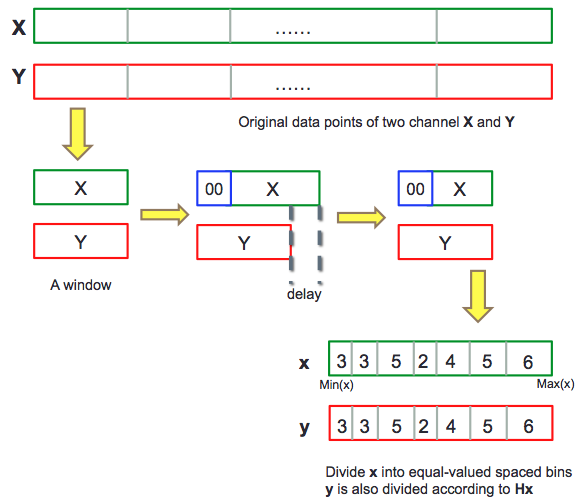
\includegraphics[width=0.45\textwidth]{./images/binsepa.png}
    \caption{An example of separating EEG time series into windows and bins for computing the nonlinear regression curves}
    \label{fig:bin}
\end{figure}
Suppose we have two channels of EEG signals $x$ and $y$, nonlinear regression analysis provides a measure called \emph{correlation ratio} $\eta^2$, whose estimator is called $h^2$. $\eta^2$ (or $h^2$) gives a statistical measure that describes the dependency of signal $x$ on $y$. Assume the amplitude of signal $y$ is a function of the amplitude of signal $x$. The expectation of $y$ given a value of $x$ is denoted as $\mu_{y|x}$ where:
\begin{equation} \label{eq:regressioncurve}
\mu_{y|x} = \int_{-\infty}^{\infty} y p(y|x) \mathrm{d}y
\end{equation}
$\mu_{y|x}$ describes the predicted value of $y$ given $x$. By this definition, we can calculate $\eta^2$, which represents the reduction of variance of $y$ that obtained by predicting $y$ value using $\mu_{y|x}$. $\eta^2$ is expressed as:
\begin{equation} \label{eq:NRAregression}
\eta^2 = \frac{Total \ Variance - Unexplained \ Variance}{Total \ Variance}
\end{equation}
Explained variance is the variance calculated from $y$ according to $\mu_{y|x}$. In this paper, nonlinear regression analysis algorithm is implemented by fieldtrip toolbox\copyright.

\subsection{Significance Check}
The significance check runs for the same processes for both methods (Grancer causality and Nonlinear Regression Analysis) and is split into two main parts: (1) p-value calculation for samples based on theoretical asymptotic null distribution; (2) statistical significance adjusted for \emph{Bonfferroni} correction.

The \emph{null hypothesis} $H_0$ is set to "there is no functional connectivity between two channels". The final conclusion after the test is given in terms of the \emph{null hypothesis}, i.e. we either \emph{reject $H_0$} or \emph{do not reject $H_0$}. In this paper, we assume that the connectivity values come from normal distribution with known mean and standard deviation and set the $p-value$ to 0.05 for testing threshold. We used $F$ test for estimating $p-value$ for functional connectivity maps estimated from Granger Causality and Nonlinear Regression Analysis models because $F$ test is commonly used to compare between two models and test which model is statistically better from another.

\subsection{Network Feature Extraction}
The functional connectivity maps gives us a view of how channels communicate information with each other, thus we can consider this map as a kins of network. In this case, we can apply network features to analyse our functional connectivity maps. Different view of treating brain networks has been proposed by different groups. Some research group see the brain network as a kind of scale-free network~\cite{eguiluz2005scale} while some others view it as a small-world network~\cite{bassett2006small}. In this section, we introduced two categories of network features, according to both scale-free network and small-world network, used in this paper -- \emph{physical statistics} feature for scale-free network and \emph{graph theory-based} feature for small-world network.

\subsubsection{Small-World Network Features}
A small-world network is a kind of network with its nodes are not neighbours of one another but most of them can be reached from every others by a small number of steps. The brain is considered as a small-world network~\cite{bassett2006small} because of the  following three reasons.

(a) The brain is a complex network on multiple spatial and time scales. Since small-world network properties occurs in many other complex networks over a wide range of physical scales, we can also consider brain as a small-world network.

(b) The brain supports both segregated and distributed information processing. Small-world topology can comprise both high clustering (segregated processing) and short path length (distributed processing).

(c) The brain likely evolved to maximise efficiency and minimise the costs of information processing. Small-world topology can operate dynamically in a critical state, facilitating rapid adaptive reconfiguration of neuronal assemblies in support of changing cognitive states.

Different aspects of small-world network has been studied and here, based on the commonly used features in neural network studies, we introduce four features for analysing our functional connectivity maps which are \emph{characteristic path}, \emph{global efficiency}, \emph{local efficiency} and \emph{clustering coefficient}~\cite{watts1998collective}~\cite{latora2001efficient}.

Characteristic path represents the averaged shortest path over the network, which will reach its minimum value when the network is a complete graph (every pair of distinct vertices is connected by a unique edge). In our case, we can interpret the characteristic path as a feature presenting the number of connections in the functional connectivity networks. The more connections exist in the functional connectivity network, the smaller value of characteristic path length is, thus the faster information can be transferred through the network. The concept of global efficiency of a small-world network is introduced by Latora and Marchiori~\cite{latora2001efficient}, provides a measure of efficient behaviour of the network by assuming that the network system is parallel (every vertex sends information concurrently through its edges in the network). It shows that with shorter characteristic path of each connection, the global efficiency of the network will be higher. It measures how efficiently the vertices exchange information through the network concurrently. With the definition of global efficiency, we can also give the definition of local efficiency by measuring the averaged efficiency of the sub-graphs \textbf{$G_i$} of the neighbours of vertex $i$ in the graph. Since the sub-graphs \textbf{$G_i$} do not contain vertex $i$, it can show how efficient the communication is when $i$ is removed from the network. Thus the local efficiency $E_{loc}$ reveals how much the network is fault tolerant. Cluster coefficient of a network measures the degree to which vertices in a graph tend to cluster together. The overall level of clustering in a network measurement is given by Watts and Strogatz~\cite{watts1998collective} as the average of the local clustering coefficients of all vertices. 

\subsubsection{Scale-Free Network Features}
Although graph theory has been successfully used to describe brain functional connectivity networks, a few studies have shown that brain functional connectivity can also be considered as a scale-free network. A scale-free network is defined as a network whose degree distribution follows a power law, which is the fraction $P(k)$ of nodes in the network having $k$ connections to other nodes goes for a larger values of $k$ as
\begin{equation}
P(k) \sim k^{-\lambda}
\end{equation}
where $\lambda$ is a parameter valued in the range $2<\lambda<3$.
Groups of CJ Stam~\cite{stam2004functional} has found that brain functional connectivity network can be viewed as a scale-free network because the connectivity distribution followed a power-law scaling with an exponent close to 2, which suggests such functional connectivity network can be considered as a scale-free network topoloty\cite{van2008small}, detailed analysing can also be found from Thivierge's work \cite{thivierge2014scale}.

In information theory, \emph{entropy} plays an important role of measuring uncertainty. Recently, following information theoretical and statistical mechanics paradigms, several entropic measures for complexity have been proposed for network structure study and these measures have shown good performance in quantifying the level of organisation encoded in structural features of scale-free networks. It is well known that \emph{Shannon entropy} and \emph{von Neumann entropy} are related to the information present in classical and quantum systems respectively. Both of them can be used to analyse the structural feature of scale-free networks\cite{anand2009entropy}. 

The amount of Shannon entropy has a correlation with the number of network structural constraints. Examples of network constrains include: \emph{fixed number of links per vertex}, \emph{given degree sequence} (a monotonic non-increasing sequence of the degrees of vertices in the graph) and \emph{community structure} (vertices of the network can be easily grouped into sets of vertices such that each set of vertices is densely connected internally). From this point of view, we can conclude that Shannon entropy has a clear interpretation of quantifying the information presented in network structure (Detailed proof can be referred to~\cite{anand2009entropy}). The more constrains a network has, the smaller Shannon entropy it shows. This implies that if a network has a smaller Shannon entropy, it will have more constrains on the network structure, which shows this network is more optimised. Von Neumann entropy is defined by von Neumann for proving the irreversibility of quantum measurement processes at the beginning. Recently it is also shown that von Neumann entropy can also be applied to network analysis~\cite{passerini2008neumann}. It has been shown that von Neumann entropy is a measure of regularity of networks~\cite{passerini2008neumann}. For a fixed number of edges, regular networks (networks whose vertices have the same number of neighbours) have in general a higher von Neumann entropy. It is also shown that von Neumann entropy depends on the number of connected components, long paths and nontrivial symmetries. With a fixed number of edges, von Neumann entropy is smaller for networks with higher degree of cluster. The mathematical proofs can be referred to~\cite{passerini2008neumann} and~\cite{anand2009entropy}.

\subsection{Classification}

Support vector machine with a \emph{Gaussian radial basis function} kernel is used for classification. The parameter selection of $\sigma$ in RBF kernel is based on cross-validation. In particular, the dataset is split into three parts, namely training, validation and testing. Leave-one-subject-out (LOO) cross-validation is carried out to estimate the parameter $\sigma$. The testing is also carried out in a LOO cross-validation scheme. We tested 13 different values of parameter $\sigma$ ranged from 0.01 to 2. More specifically, the parameter $\sigma$ is selected based on the training and validation using data from 22 subjects, whereas one subject is left out for testing. The procedure is repeated until all subjects have been left out as test-subjects (i.e., the procedure is repeated 23 times). 

Cohen's Kappa $\kappa$~\cite{uebersax1987diversity}, is a measure of agreement between two viewers, is calculated to evaluate the classifier's performance. Some researchers consider that Cohen's kappa can be used to evaluate the agreement by chance, i.e. if the viewers are randomly guessing for a decision. In our case the two viewers actually correspond to the ground truth and test labels. Cohen's kappa is considered an accurate metric for classification performance and takes into account unbalanced classes (i.e., classes with different number of samples). 

